\documentclass[8pt]{beamer}
\usetheme{Malmoe}
\usepackage[utf8]{inputenc}
\usepackage[french]{babel}
\usepackage[T1]{fontenc}
\usepackage{amsmath}
\usepackage{amsfonts}
\usepackage{amssymb}
\usepackage{graphicx}
\usepackage{hyperref}
\author{Manon OLIVERA}
%\usecolortheme[named={white}]{structure}
\setbeamercolor{structure}{fg=blue!40!white,bg=white}
%\setbeamercovered{transparent} 
%\setbeamertemplate{navigation symbols}{} 
%\logo{} 
%\institute{} 
%\date{} 
%\subject{}

\usepackage[skins,theorems,breakable]{tcolorbox}
\usepackage{fontawesome5}
\usepackage{siunitx}
\usepackage{pstricks-add}
\usepackage{tabularx}
\usepackage{enumitem}
\usepackage{hyperref}
\usepackage{xcolor}
\usepackage{varwidth}

\setbeamertemplate{navigation symbols}{%
%\insertslidenavigationsymbol
%\insertframenavigationsymbol
%\insertsubsectionnavigationsymbol
%\insertsectionnavigationsymbol
%\insertdocnavigationsymbol
%\insertbackfindforwardnavigationsymbol
}

\newtcbtheorem{defi}{Définition\,}{
theorem style = plain, 
%oversize,
enhanced, 
breakable,
before skip = 2mm, 
after skip = 2mm, 
top = 1mm,
left = 1mm,
right = 1mm,
bottom = 1mm,
coltitle=black!50!blue,
colback=blue!5, 
colframe=blue!5,
terminator sign dash, 
fonttitle=\bfseries}{df}

\newtcbtheorem{exemple}{Exemple\,}{
theorem style = plain, 
%oversize,
enhanced, 
breakable,
before skip = 2mm, 
after skip = 2mm,
top = 1mm,
left = 1mm,
right = 1mm,
bottom = 1mm, 
coltitle=black,
colback=white, 
colframe=white,
terminator sign dash, 
fonttitle=\bfseries}{ex}

\newtcbtheorem{remarque}{Remarque\,}{
theorem style = plain, 
%oversize,
enhanced, 
breakable,
before skip = 2mm, 
after skip = 2mm,
top = 1mm,
left = 1mm,
right = 1mm,
bottom = 1mm, 
coltitle=black,
colback=white, 
colframe=white,
terminator sign dash, 
fonttitle=\bfseries}{rq}

\newtcbtheorem{prop}{Propriété\,}{
theorem style = plain, 
%oversize,
enhanced, 
breakable,
before skip = 2mm, 
after skip = 2mm, 
top = 1mm,
left = 1mm,
right = 1mm,
bottom = 1mm,
coltitle=black!50!orange,
colback=orange!5, 
colframe=orange!5,
terminator sign dash, 
fonttitle=\bfseries}{ppt}	

\newtcbtheorem{notation}{Notation\,}{
theorem style = plain, 
%oversize,
enhanced, 
breakable,
before skip = 2mm, 
after skip = 2mm,
top = 1mm,
left = 1mm,
right = 1mm,
bottom = 1mm, 
coltitle=black,
colback=white, 
colframe=white,
terminator sign dash, 
fonttitle=\bfseries}{not}

\newtcbtheorem{exercice}{Exercice}{
enhanced, 
breakable,
before skip = 2mm, 
after skip = 2mm,
top = 1mm,
left = 1mm,
right = 1mm,
bottom = 1mm, 
coltitle=white,
colbacktitle=black,
colback=white, 
colframe=black,
boxrule=0.3mm,
terminator sign none, 
fonttitle=\bfseries,
attach boxed title to top left={xshift=1cm,yshift*=1mm-\tcboxedtitleheight},
varwidth boxed title*=-3cm,
boxed title style={frame code={
            \path[fill=tcbcolback!30!black]
              ([yshift=-1mm,xshift=-1mm]frame.north west)
                arc[start angle=0,end angle=180,radius=1mm]
              ([yshift=-1mm,xshift=1mm]frame.north east)
                arc[start angle=180,end angle=0,radius=1mm];
            \path[left color=tcbcolback!60!black,right color=tcbcolback!60!black,
              middle color=tcbcolback!80!black]
              ([xshift=-2mm]frame.north west) -- ([xshift=2mm]frame.north east)
              [rounded corners=1mm]-- ([xshift=1mm,yshift=-1mm]frame.north east)
              -- (frame.south east) -- (frame.south west)
              -- ([xshift=-1mm,yshift=-1mm]frame.north west)
              [sharp corners]-- cycle;
            },interior engine=empty,
          }}{exo}

\newcommand{\cheminatome}{../atomes}

\setbeamertemplate{button}{\tikz
  \node[
  inner xsep=4pt, %largeur du bouton
  draw=structure!00, %coucleur du contour
  fill=structure!100, %transparence
  rounded corners=6pt]  {\large\insertbuttontext};}
  
\title{Chapitre N1 - Nombres entiers}

\begin{document}

\begin{frame}
\titlepage
\end{frame}

\begin{frame}

\hypertarget{menu}{ }

\hfill
\hyperlink{debat}{\begin{tcolorbox}[width=3cm,height= 1.5cm,left=1mm,right=1mm,top=1mm,bottom=1mm,nobeforeafter,enhanced,drop fuzzy shadow southeast,valign=center,halign=center,colframe=blue!10!white,colback=blue!10!white] 
\textbf{{\LARGE Débat}} 
\end{tcolorbox}}
\hfill
\hyperlink{activite}{\begin{tcolorbox}[width=3cm,height= 1.5cm,left=1mm,right=1mm,top=1mm,bottom=1mm,nobeforeafter,enhanced,drop fuzzy shadow southeast,valign=center,halign=center,colframe=green!10!white,colback=green!10!white]
\textbf{{\LARGE Activité}}
\end{tcolorbox}}
\hfill \,

\vspace{1cm}

\hfill 
\hyperlink{cours}{\begin{tcolorbox}[width=3cm,height= 1.5cm,left=1mm,right=1mm,top=1mm,bottom=1mm,nobeforeafter,enhanced,drop fuzzy shadow southeast,valign=center,halign=center,colframe=orange!10!white,colback=orange!10!white] 
\textbf{{\LARGE Cours}} 
\end{tcolorbox}}
\hfill \,

\vspace{1cm}

\hfill 
\hyperlink{exercices}{\begin{tcolorbox}[width=3cm,height= 1.5cm,left=1mm,right=1mm,top=1mm,bottom=1mm,nobeforeafter,enhanced,drop fuzzy shadow southeast,valign=center,halign=center,colframe=red!10!white,colback=red!10!white] 
\textbf{{\LARGE Exercices}} 
\end{tcolorbox}} 
\hfill 
\hyperlink{recreation}{\begin{tcolorbox}[width=3cm,height= 1.5cm,left=1mm,right=1mm,top=1mm,bottom=1mm,nobeforeafter,enhanced,drop fuzzy shadow southeast,valign=center,halign=center,colframe=pink!30!white,colback=pink!30!white] 
\textbf{{\LARGE Récréation}} 
\end{tcolorbox}} 
\hfill \,

\end{frame}

\begin{frame}
\frametitle{\hypertarget{debat}{\textbf{Débat}} \hspace{0pt plus 1 filll} \hyperlink{menu}{\beamerbutton{\faHome}}}
\begin{center}
\href{https://www.youtube-nocookie.com/embed/WRrLnktqUmE?playlist=WRrLnktqUmE&autoplay=1&iv_load_policy=3&loop=1&modestbranding=1&start=}{
\includegraphics[scale=0.6]{video.jpg}}
\end{center}
\end{frame}

\begin{frame}
\frametitle{\hypertarget{activite}{\textbf{Activité}} \hspace{0pt plus 1 filll} \hyperlink{menu}{\beamerbutton{\faHome}}}
\begin{center}
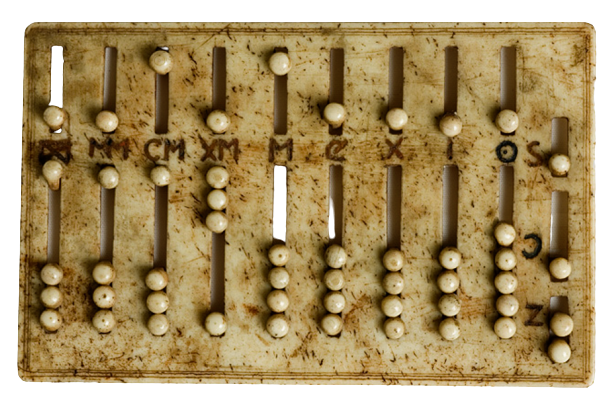
\includegraphics[scale=0.8]{abaque.png} 
\end{center}
\end{frame}

\begin{frame}
\frametitle{\hypertarget{cours}{\textbf{Chapitre N1 : Nombres entiers}} \hspace{0pt plus 1 filll} \hyperlink{menu}{\beamerbutton{\faHome}}}
\begin{Large}
\hyperlink{section1}{1. Écriture des nombres entiers} \\
\vspace{5mm}
\hyperlink{section2}{2. La règle graduée} \\
\vspace{5mm}
\hyperlink{section3}{3. Ordonner des nombres entiers}
\end{Large}
\end{frame}

\begin{frame}
\frametitle{1. Écriture des nombres entiers \hypertarget{section1}{ } \hspace{0pt plus 1 filll} \hyperlink{cours}{\beamerbutton{\faReply}} {\Huge \textcolor{blue!10!white}{\faAngleLeft}} \hyperlink{menu}{\beamerbutton{\faHome}} \hyperlinkslidenext{{\Huge \faAngleRight}}} 
\begin{defi*}{}{}
Dans notre numération, il y a dix \textbf{chiffres} : 0, 1, 2, 3, 4, 5, 6, 7, 8 et 9. Ces chiffres permettent d'écrire des \textbf{nombres entiers} : il y en a une infinité.
\end{defi*}

\begin{exemple*}{}{}
\num{1054} est un nombre composé de quatre chiffres. 7 est un nombre composé d'un seul chiffre.
\end{exemple*}
\end{frame}

\begin{frame}
\frametitle{ \hspace{0pt plus 1 filll} \hyperlink{cours}{\beamerbutton{\faReply}} \hyperlinkslideprev{{\Huge \faAngleLeft}} \hyperlink{menu}{\beamerbutton{\faHome}} \hyperlinkslidenext{{\Huge \faAngleRight}}} 
\begin{defi*}{}{}
Les nombres sont regroupés en \textbf{classes} composées de trois rangs : unités, dizaines, centaines. On peut représenter ces données dans un tableau.

\renewcommand{\arraystretch}{1.8}
\begin{center}
    \scalebox{0.8}{
    \begin{tabular}{*{3}{|c}|*{3}{|c}|*{3}{|c}|*{3}{|c}|}
        \hline
        \multicolumn{3}{|c||}{\textbf{Classe des Milliards}} & \multicolumn{3}{c||}{\textbf{Classe des Millions}}&\multicolumn{3}{c||}{\textbf{Classe des Milliers}}&\multicolumn{3}{c|}{\textbf{Classe des Unités}}\\
        \hline
        \rotatebox{90}{\parbox{3.5cm}{\textbf{Centaines}\\ de milliards }}& 
        \rotatebox{90}{\parbox{3.5cm}{\textbf{Dizaines}\\ de milliards }}& 
        \rotatebox{90}{\parbox{3.5cm}{\textbf{Unités}\\ de milliards }}& 
        \rotatebox{90}{\parbox{3.5cm}{\textbf{Centaines}\\ de millions }}& 
        \rotatebox{90}{\parbox{3.5cm}{\textbf{Dizaines}\\ de millions }}& 
        \rotatebox{90}{\parbox{3.5cm}{\textbf{Unités}\\ de millions }}& 
        \rotatebox{90}{\parbox{3.5cm}{\textbf{Centaines}\\ de milliers }}& 
        \rotatebox{90}{\parbox{3.5cm}{\textbf{Dizaines}\\ de milliers }}& 
        \rotatebox{90}{\parbox{3.5cm}{\textbf{Unités}\\ de milliers }}& 
        \rotatebox{90}{\parbox{3.5cm}{\textbf{Centaines}\\ d'unités }}& 
        \rotatebox{90}{\parbox{3.5cm}{\textbf{Dizaines}\\ d'unités }}&
        \rotatebox{90}{\parbox{3.5cm}{\textbf{Unités}\\ d'unités}} 
        \\
        \hline
        & & & & 1 & 2 & 0 & 4 & 5 & 9 & 7 & 6 \\
        \hline
    \end{tabular} 
    }
   \end{center}
\end{defi*}
   
\begin{exemple*}{}{}
Dans le nombre \num{12045976} :
\begin{itemize}[label=$-$]
\begin{minipage}[t]{0.55\linewidth}
	\item 9 est le chiffre des centaines ;
	\item 5 est le chiffre des milliers ;
	\item 1 est le chiffre des dizaines de millions ;
\end{minipage}
\begin{minipage}[t]{0.38\linewidth}
	\item il y a \num{120459} centaines ;
	\item il y a \num{1204} dizaines de milliers ;
	\item il y a 12 millions.
\end{minipage}
\end{itemize}
\end{exemple*}
\end{frame}

\begin{frame}
\frametitle{ \hspace{0pt plus 1 filll} \hyperlink{cours}{\beamerbutton{\faReply}} \hyperlinkslideprev{{\Huge \faAngleLeft}} \hyperlink{menu}{\beamerbutton{\faHome}} \hyperlinkslidenext{{\Huge \faAngleRight}}}
\begin{defi*}{}{}
On peut décomposer tout nombre sous sa \textbf{forme canonique} :
\begin{align*}
\num{12045976} = \; &\num{10000000} + \num{2000000} + \num{40000} + \num{5000} + 900 + 70 + 2 \\
= \; &(1\times\num{10000000}) + (2\times\num{1000000}) + (4\times\num{10000}) + (5\times\num{1000}) \\
\; &+ (9\times100) +(7\times10) + ( 6\times1)
\end{align*}
\end{defi*}
\end{frame}

\begin{frame}
\frametitle{ \hspace{0pt plus 1 filll} \hyperlink{cours}{\beamerbutton{\faReply}} \hyperlinkslideprev{{\Huge \faAngleLeft}} \hyperlink{menu}{\beamerbutton{\faHome}} \hyperlinkslidenext{{\Huge \faAngleRight}}}
\begin{prop*}{}{}
Pour pouvoir lire les grands nombres plus facilement, on regroupe les chiffres par tranches de trois en partant du chiffre des unités de la classe des unités.
\end{prop*}

\begin{exemple*}{}{}
\begin{itemize}[label=$-$]
	\item $12345678910111213$ s'écrira plutôt $\num{12345678910111213}$.
	\item $9123456789$ s'écrira plutôt $\num{9123456789}$, et se lit \og neuf \underline{milliards} cent vingt-trois \underline{millions} quatre cent cinquante-six \underline{mille} sept cent quatre-vingt-neuf \underline{unités} \fg
\end{itemize}
\end{exemple*}
\end{frame}

\begin{frame}
\frametitle{ \hspace{0pt plus 1 filll} \hyperlink{cours}{\beamerbutton{\faReply}} \hyperlinkslideprev{{\Huge \faAngleLeft}} \hyperlink{menu}{\beamerbutton{\faHome}} \hyperlinkslidenext{{\Huge \faAngleRight}}}
\begin{prop*}{Règles orthographiques}{}
\begin{itemize}[label=$-$]
	\item Deux mots d'un même nombre sont séparés par un trait d'union.
	\item \og Mille \fg \, est invariable.
	\item \og Cent \fg \, ou \og vingt \fg \, prennent la marque du pluriel, \og s \fg, sauf quand ils sont suivis d'un autre adjectif numéral (\og quatre \fg{} par exemple). Toutefois, devant \og millier \fg, \og million \fg \, ou \og milliard \fg, qui sont des noms, le \og s \fg \, du pluriel subsiste.
	\item \og Million \fg \, et \og milliard \fg \, prennent toujours un \og s \fg{} quand ils sont au pluriel.
\end{itemize}
\end{prop*}

\begin{exemple*}{}{}
\begin{itemize}[label=$-$]
	\item \num{4000} : quatre-mille ;        
	\item \num{12045976} : douze-millions-quarante-cinq-mille-neuf-cent-soixante-seize.
	\item $80$ s'écrit "quatre-vingt\underline{s}" mais $83$ s'écrit "quatre-vingt-trois"
	\item $200$ s'écrit "deux-cent\underline{s}" mais $237$ s'écrit "deux-cent trente-sept"
	\item Deux-cents personnes sont attendues, mais établissez un chèque de cinq-cent quarante euros
\end{itemize}
\end{exemple*}
\end{frame}

\begin{frame}[t]
\frametitle{2. La règle graduée \hypertarget{section2}{ } \hspace{0pt plus 1 filll} \hyperlink{cours}{\beamerbutton{\faReply}} \hyperlinkslideprev{{\Huge \faAngleLeft}} \hyperlink{menu}{\beamerbutton{\faHome}} \hyperlinkslidenext{{\Huge \faAngleRight}}}
\begin{defi*}{}{}
Pour graduer une droite, il faut choisir :
\begin{itemize}[label=$-$]
	\item une {\bf origine} qui correspond au \og 0 \fg{},
	\item une {\bf unité} qui sera reportée de manière régulière,
	\item un {\bf sens croissant}.
\end{itemize}
Un point est repéré par son {\bf abscisse}. A a pour abscisse 3 se note A(3).
\end{defi*}

\end{frame}

\begin{frame}
\frametitle{3. Ordonner des nombres entiers\hypertarget{section3}{ } \hspace{0pt plus 1 filll} \hyperlink{cours}{\beamerbutton{\faReply}} \hyperlinkslideprev{{\Huge \faAngleLeft}} \hyperlink{menu}{\beamerbutton{\faHome}} \hyperlinkslidenext{{\Huge \faAngleRight}}}
\begin{defi*}{}{}
{\bf Comparer} deux nombres, c'est dire s'ils sont égaux ou si l'un est plus petit (ou plus grand) que l'autre.
\end{defi*}

\begin{notation*}{}{}
Dans notre sens de lecture (de gauche à droite), le symbole \fbox{<} signifie \og plus petit que \fg{} et \fbox{>} signifie \og plus grand que \fg{}.  
\end{notation*}

\begin{exemple*}{}{}
\begin{itemize}[label=$-$]
	\item $\num{1000000200} > \num{1000000002}$ se lit \og $\num{1000000200}$ est plus grand que $\num{1000000002}$ \fg{}. 
	\item $\num{999999}<\num{1000000}$ si lit \og $\num{999999}$ est plus petit que $\num{1000000}$ \fg{}.
\end{itemize}
\end{exemple*}
\end{frame}

\begin{frame}
\frametitle{ \hspace{0pt plus 1 filll} \hyperlink{cours}{\beamerbutton{\faReply}} \hyperlinkslideprev{{\Huge \faAngleLeft}} \hyperlink{menu}{\beamerbutton{\faHome}} \hyperlinkslidenext{{\Huge \faAngleRight}}}
\begin{defi*}{}{}
\begin{itemize}[label=$-$]
	\item Ranger des nombres dans l'ordre {\bf croissant} signifie les ranger du plus petit au plus grand.
	\item Ranger des nombres dans l'ordre {\bf décroissant} signifie les ranger du plus grand au plus petit.
\end{itemize}
\end{defi*}

\begin{exemple*}{}{}
\begin{itemize}[label=$-$]
	\item $\num{1000045}<\num{1000085}<\num{1000600}<\num{1000607}$ sont rangés dans l'ordre croissant.
	\item $321>312>231>213>132>123$ sont rangés dans l'ordre décroissant.
	\end{itemize}
\end{exemple*}
\end{frame}

\begin{frame}
\frametitle{ \hspace{0pt plus 1 filll} \hyperlink{cours}{\beamerbutton{\faReply}} \hyperlinkslideprev{{\Huge \faAngleLeft}} \hyperlink{menu}{\beamerbutton{\faHome}} {\Huge \textcolor{blue!10!white}{\faAngleRight}}}
\begin{defi*}{}{}
{\bf Encadrer} un nombre, c'est l'entourer par un nombre plus petit et un nombre plus grand.
\end{defi*}

\begin{exemple*}{}{}
On peut encadrer le nombre 8\,199 de différentes façons, par exemple :   
\begin{itemize}
	\item $\num{8198}<\num{8199}<\num{8200}$
	\item $\num{8000}<\num{8199}<\num{9000}$
	\item $\num{1000}<\num{8199}<\num{10000}$\dots
\end{itemize}
\end{exemple*}
\end{frame}

\begin{frame}
\frametitle{\hypertarget{exercices}{\textbf{Exercices}} \hspace{0pt plus 1 filll} \hyperlink{menu}{\beamerbutton{\faHome}}}
\begin{Large}
\hyperlink{section1exo}{1. Écriture des nombres entiers} \\
\vspace{5mm}
\hyperlink{section2exo}{2. La règle graduée} \\
\vspace{5mm}
\hyperlink{section3exo}{3. Ordonner des nombres entiers}
\end{Large}
\end{frame}

\begin{frame}
\frametitle{\hypertarget{section1exo}{1. Écriture des nombres entiers} \hspace{0pt plus 1 filll} \hyperlink{exercices}{\beamerbutton{\faReply}} {\Huge \textcolor{blue!10!white}{\faAngleLeft}} \hyperlink{menu}{\beamerbutton{\faHome}} \hyperlinkslidenext{{\Huge \faAngleRight}}}
\begin{exercice}{}{}
Écrire en chiffre les nombres suivants :
\begin{enumerate}
	\item Sept-milliards-cinq-cent-cinquante-neuf-millions-deux-cent-quatre-vingt-huit-mille-trois-cents.
	\item Neuf-millions-sept-cent-mille-sept-cent-quarante. 
   \item Trente-huit-millions-trente-huit-mille.
   \item Vingt-six-milliards-cent-huit-millions-sept-cent-vingt-huit-mille-douze.
\end{enumerate}
\end{exercice}
\end{frame}

\begin{frame}[t]
\frametitle{\hypertarget{recreation}{\textbf{Récréation}} \hspace{0pt plus 1 filll} \hyperlink{menu}{\beamerbutton{\faHome}}}
\end{frame}

\end{document}